\documentclass[11pt]{article}

\usepackage{fancyhdr}
\usepackage[a4paper,tmargin=15mm,lmargin=27mm,bmargin=15mm,rmargin=27mm,verbose,showframe]{geometry}
\usepackage{float}
\usepackage{tikz}

\usepackage{ifthen}
\usepackage{forloop}
\usepackage{lipsum}

\setlength{\parindent}{0pt}

\begin{document}


\begin{tikzpicture}[every circle node/.style={circle, draw, black, very thick, line width=12pt, inner sep=4mm}]
    \node[circle] at (0,0) {};
    \node[circle] at (14,0) {};
\end{tikzpicture}

% \lipsum[1-5]

% Include WSU logo
\begin{figure}[h]
    \centering
    \includegraphics[height=30mm]{WSUI_Logo.png}
\end{figure}

\begin{center}
    {\Large\textbf{Multiple Choice Scan Sheet}}
\end{center}

\fbox{
    \begin{minipage}{50mm}
        \newcounter{i}
        \forloop{i}{1}{\value{i} < 31}{
            \hspace*{1em}
            \ifthenelse{\value{i} < 10}{\hspace*{6pt}}{}
            \arabic{i})
            \scalebox{0.5}{
                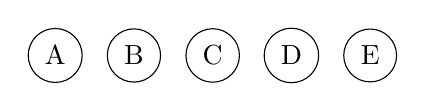
\begin{tikzpicture}[every circle node/.style={circle, draw, thin}]
                    \node[circle] at (0,0) {A};
                    \node[circle] at (1,0) {B};
                    \node[circle] at (2,0) {C};
                    \node[circle] at (3,0) {D};
                    \node[circle] at (4,0) {E};
                \end{tikzpicture}
            }
            \\
        }
    \end{minipage}
}
\hspace{10mm}
\fbox{
    \begin{minipage}{80mm}
        \begin{tabular}[ht]{r l}
            Subject Code: & \rule[-1pt]{45mm}{1pt} \\\\
            Date: & \rule[-1pt]{45mm}{1pt} \\\\
            Student Name: & \rule[-1pt]{45mm}{1pt} \\\\
        \end{tabular}
        \vspace{3mm}
        
        \newcounter{j}
        \newcounter{k}
        \forloop{j}{0}{\value{j} < 9}{
            % \arabic{j})
            \ifthenelse{\equal{\value{j}}{0}}{
                    \hspace{4mm}\textbf{ID}\hspace{2.2mm}
                    \forloop{k}{0}{\value{k} < 10}{\hspace{1mm}\textbf{\arabic{k}}\hspace{2.8mm}}
                }
                {
                    \scalebox{0.6}{
                        \begin{tikzpicture}[
                                every rectangle node/.style={rectangle, draw, thin, minimum width=17mm, minimum height=7mm},
                                every circle node/.style={circle, draw, thin}
                            ]
                            \node[rectangle] at (0,\value{j}) {};
                            \hspace{5mm}
                            \forloop{k}{0}{\value{k} < 10}{
                                \node[circle] at (\value{k}+1,\value{j}) {\arabic{k}};
                            }
                        \end{tikzpicture}
                    }
                }
            \vspace{1.5mm}
            \\
        }
    \end{minipage}
}

\vspace{20mm}
\bigskip


\begin{tikzpicture}[every circle node/.style={circle, draw, black, very thick, line width=12pt, inner sep=4mm}]
    \node[circle] at (0,0) {};
    \node[circle] at (14,0) {};
\end{tikzpicture}

\end{document}